\documentclass{article}
%\usepackage[hscale=.85,vscale=.9]{geometry}                % See geometry.pdf to learn the layout options. There are lots.

\usepackage{adjmulticol}
\usepackage[a4paper, landscape, margin=2.5cm]{geometry}
\usepackage{graphicx}
\usepackage{amssymb}
\usepackage{epstopdf}
\usepackage{lmodern} 
\usepackage{xcolor} 

\DeclareGraphicsRule{.tif}{png}{.png}{`convert #1 `dirname #1`/`basename #1 .tif`.png}

\usepackage{newpxtext} 
\usepackage{newpxmath}

\pagestyle{empty}

\advance \textwidth by 1in
\advance \leftmargin by -1in
\advance \topmargin by -1cm
\advance \textheight by 2cm

\begin{document}
%\drawfoldlines

\setlength{\columnsep}{2cm}

\begin{adjmulticols}{3}{-1cm}{1cm}

\hskip 77mm \setbox0 = \hbox{\raise 1cm\hbox{\vrule height 3cm depth 20cm width .5pt}} \ht0=0pt \dp0=0pt \copy0

\leavevmode
\vskip -6ex
\begin{center}\vskip -3ex\leavevmode\hbox{\fontsize{26}{15}\selectfont\sf\bfseries
\textcolor{blue}{The   Game   of   Life}}\end{center}
\vskip 2ex
\begin{center}
\fontsize{12}{40}\selectfont
\def\s{\hskip .3ex}
\def\dot#1{\includegraphics[width=0.5cm]{#1}}
\dot{blend1.png} \s
\dot{blend2.png} \s
\dot{blend3.png} \s
\dot{blend4.png} \s
\dot{blend5.png} \s
\dot{blend6.png} \s
\dot{blend7.png} \s
\dot{blend8.png} \s
\dot{blend9.png} \s
\dot{blend10.png} \s
\\
\dot{blend11.png} \s
\dot{blend12.png} \s
\dot{blend13.png} \s
\dot{blend14.png} \s
\dot{blend15.png} \s
\dot{blend16.png} \s
\dot{blend17.png} \s
\dot{blend18.png} \s
\dot{blend19.png} \s
\dot{blend20.png}

\fontsize{12}{14}\selectfont
%\vskip -2ex\em Simple rules get surprising effects
\end{center}

\vskip 0cm

\def\sec#1{\vskip 3ex
	\fontsize{23}{26}\selectfont\noindent
	\textcolor{red}{\textsf{\bfseries #1}}\fontsize{15}{18}\selectfont
	\vskip 2ex
	\noindent
}
\def\liferule#1{\vskip 3ex
	\fontsize{18}{16}\selectfont\noindent
	\textcolor{blue}{\textsf{\bfseries #1}}\fontsize{15}{18}\selectfont
	\vskip 2ex
	\noindent
}
\def\in{~~~~}
\fontsize{15}{18}\selectfont
\raggedright\vskip 4ex
\noindent
{\sf When I was 15 I got interested in John Conway's Game of Life reading an article about it in the October 1970 issue of the \emph{Scientific American\/} magazine.}

\vskip 18ex\begin{center}
\framebox{\begin{minipage}{.9\linewidth}\begin{center}
Harold Thimbleby
\vskip 1ex
\texttt{harold@thimbleby.net}
\vskip 1ex
July 2026
\end{center}\end{minipage}}\end{center}

\newcolumn
\sec{Computers, free will, \\and your mind}

%You can imagine Game of Life gliders carrying messages, and indeed people have used them to actually send messages across large game boards, just like sending signals along wires. 

The Game of Life has figured in a lot of arguments about free will. 

\in Many people argue the Game of Life has free will because \emph{in principle\/} it is unpredictable. But being unpredictable means the patterns must also be unpredictable \emph{to themselves}, which isn't what I take free will to mean.

\in Although a single brain synapse or neuron can't do much more than a cell in the Game of Life, your amazing brain has around 1,000~trillion (1,000,000,000,000,000) synapses all working together, ending up with the miraculous complexity of all your memories, your thinking, and your appreciation of science and art.

\newcolumn
\in  With only 150 times more cells than than this exhibit, the Game of Life can simulate 
a fully-working programmable computer.

\in It's a challenging thought that if the Game of Life was scaled up to millions of cells it would be capable of artificial intelligence, and it could be made so tiny  many would fit on a pin head.

\in One of my favourite examples of how surprising the Game of Life is is that the Game of Life can play the Game of Life itself. 

\in That's a bit like what your own consciousness does when you think about yourself. So, does that mean the Game of Life can be conscious too? 

\in There are no scientific reasons why not, but its consciousness would be very different from ours.

\vskip 1cm\noindent\framebox{\begin{minipage}{\linewidth}
\fontsize{10}{13}\selectfont
Download links and the open source Python \hbox{program} I wrote to run the Game of Life at:\\
\texttt{https://www.harold.thimbleby.net/life}
\end{minipage}}

\newcolumn\sec{Very simple rules}

%The Game of Life has simple rules, but very complicated things can happen very quickly. Cells can be `dead' or `alive.' In this display, each live cell is shown by a round stone. 

%\in 
This small exhibit is enough to show how complexity can emerge from simple rules. 

%\in Here are \emph{all\/} the rules of the Game of Life: 

\in Each cell in the Game of Life is surrounded by up to eight other neighbouring cells, which may be dead or alive.

\vskip 1cm\begin{center}
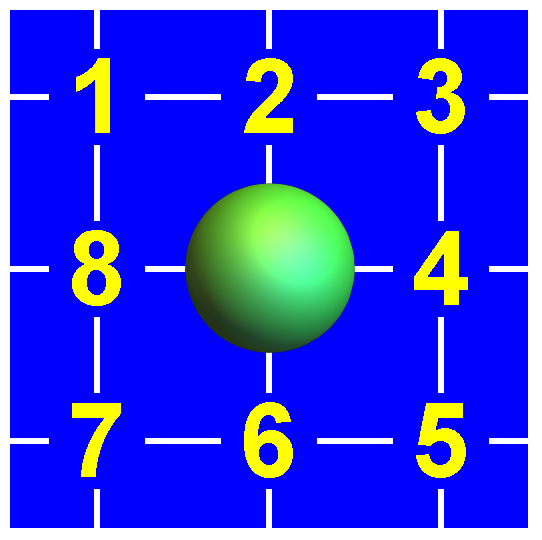
\includegraphics[width=.8\columnwidth]{grid.pdf}
\end{center}
\vskip 1cm

\in In the exhibit here, newborn cells are green, and as they age they are turned red then brown then black, like autumn leaves.
\noindent
\def\gap{\hbox to 0in{}}

\newcolumn
\sec{Just four rules}

{\liferule{\bfseries 1 Under-population}\\ \sf Any live cell with fewer than two live \hbox{neighbours} dies.\\
\liferule{\bfseries 2 Survival}\\ \sf Any live cell with two or three live \hbox{neighbours} lives on to the next \hbox{generation}.\\
\liferule{\bfseries 3 Reproduction}\\ \sf Three live neighbours reproduce to \hbox{create} a new live cell.\\
\liferule{\bfseries 4 Over-population}\\ \sf Any live cell with more than three live neighbours dies.
}\vskip 1.2cm

\hrule height 2pt 
\vskip 2mm\in \textbf{That's all there is to it.}
\vskip 2mm\hrule height 2pt 

\newcolumn

\in In the exhibit here the rules are run every fraction of a second to create a new generation, using a Raspberry Pi computer behind the scenes. 

\in If you watch the exhibit, you can see how the rules work. 

\in 
The Game of Life is so popular people spend their time looking for interesting patterns.  Bill Gosper discovered the first ``glider gun'' in 1970 which fires off lots of ``gliders.'' The exhibit here shows a glider gun, some gliders, and a few other popular life forms.
%One of Gosper's glider guns is shown at the top of our pre-planned show. You can see it repeatedly shooting gliders diagonally towards the bottom of the display.

\in The traffic lights (bottom left of the pre-planned show, and often found somewhere on the random show) are a good place to appreciate how the simple rules can create action.

\vfill
\textbf{Email me, or see the Wikipedia article \emph{Conway's Game of Life} for lots more info.}


\end{adjmulticols}

\end{document}  